\section{倒立振子のモデリング}
実験目的を達成する制御システムを設計するためにまず、倒立振子系について、状態方程式と観測方程式から成る数式モデルを導出する。
\subsection{状態方程式}
	\begin{figure}[H]
		\centering
		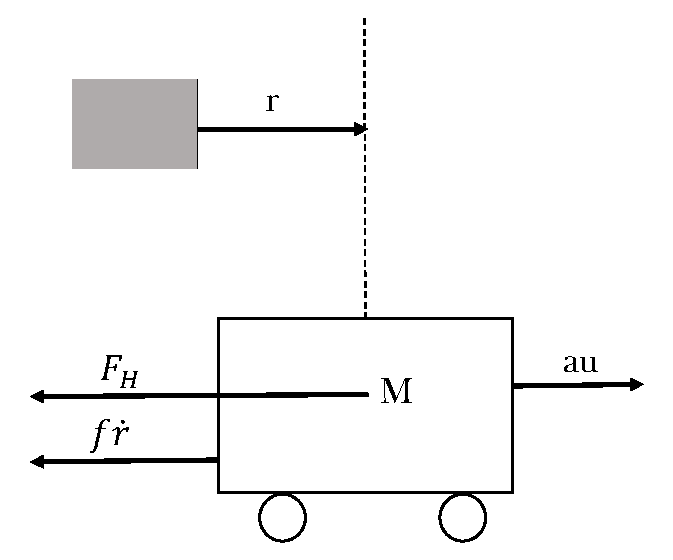
\includegraphics[width=0.4\linewidth]{gazo/cart.eps}
		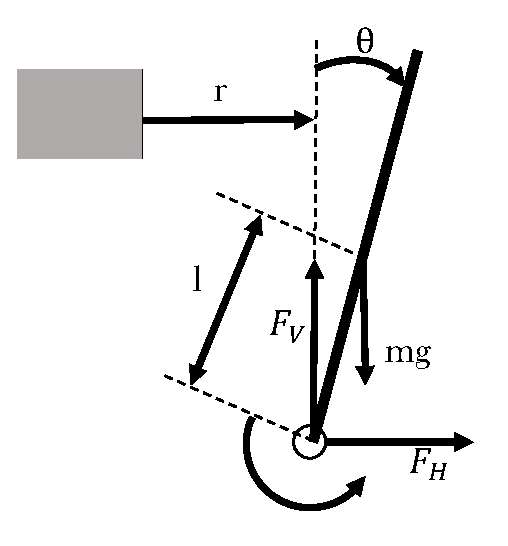
\includegraphics[width=0.4\linewidth]{gazo/stick.eps}
		\caption{数式モデル導出のための参考図}
		\label{image:reference}
	\end{figure}	
	図\ref{image:reference}を参考に各運動方程式を導出すると、\\
	台車の運動方程式は\\
	
	\begin{equation}
		M\ddot{r}=au-F_{H}-f\dot{r}
		\label{eq:motion_eq_cart}
	\end{equation}
	\\
	倒立振子の回転の運動方程式は\\
	
	\begin{equation}
		J\ddot{\theta}=lF_{V}\sin \theta -lF_{H}\cos \theta -c\dot{\theta}
		\label{eq:rotemotion_eq_stick}
	\end{equation}
	\\
	倒立振子の水平方向の運動方程式は\\
	
	\begin{equation}
		m\frac{d^{2}}{dt^{2}}(r+l\sin\theta) = F_{H}
		\label{eq:horizonmotion_eq_stick}
	\end{equation}
	\\
	倒立振子の垂直方向の運動方程式は\\
	
	\begin{equation}
		m\frac{d^{2}}{dt^{2}}(l\cos\theta) = F_{V}-mg
		\label{eq:vertical_eq_stick}
	\end{equation}
	
	となる。
	\par
	ここで各式の導出過程を述べる。図\ref{image:reference}より台車の運動方程式は、振り子からの水平抗力$F_{H}$を考慮してニュートンの第二法則より(\ref{eq:motion_eq_cart})
	式を導くことができる。
	ただし、$M$は台車の質量、$f$は台車の摩擦係数、$a$は駆動アンプへの入力電圧から台車への駆動までのゲイン、$u$はモータの駆動アンプへの入力電圧、$r$は台車の基準位置からの変位である。
	同様にニュートンの第二法則を用いることで(\ref{eq:horizonmotion_eq_stick}),(\ref{eq:vertical_eq_stick})式の運動方程式を導くことができる。
	ただし、$m$は振り子の質量、$l$は回転軸・重心間の距離、$g$は重力加速度、$F_{V}$は振り子が台車から受ける垂直抗力である。
	また、$\theta$は鉛直上向きを$\theta=0$としたときの角度である。
	最後に(\ref{eq:rotemotion_eq_stick})式は回転に対する運動方程式を考えることで上記と同様に求めることができる。
	ただし、$J$は重心回りの慣性モーメント、$c$は回転軸摩擦係数である。
	\par
	いま、4つの状態変数から成るベクトル、すなわち状態$x$を
					
	\begin{eqnarray}
		x=\left[
		\begin{array}{ccc}
			r\\
			\theta\\
			\dot{r}\\
			\dot{\theta}\\
		\end{array}
		\right]
		\label{eq:array1}
	\end{eqnarray}
					
	のように定義し、(\ref{eq:motion_eq_cart}),(\ref{eq:rotemotion_eq_stick}),
	(\ref{eq:horizonmotion_eq_stick}),(\ref{eq:vertical_eq_stick})
	式から倒立振子系の非線形状態方程式を求める。
	\begin{eqnarray}
		\dot{x} = f(x,u) = \left[
		\begin{array}{ccc}
			\dot{r}\\
			\dot{\theta}\\
			\ddot{r}\\
			\ddot{\theta}\\
		\end{array}
		\right]
		\label{eq:array2}
	\end{eqnarray}
					
	ここで(\ref{eq:horizonmotion_eq_stick})式より$F_{H}$を、
	(\ref{eq:vertical_eq_stick})式より$F_{V}$を求めると
	
	\[F_{H} = m\frac{d^{2}}{dt^{2}}r + ml\frac{d^{2}}{dt^{2}}\sin{\theta}\]
	\begin{equation}
		= m\ddot{r}+ml(-\dot{\theta}^{2}\sin{\theta}+\ddot{\theta}\cos{\theta})
		\label{eq:eq1}
	\end{equation}
	\\
	\[F_{V} = mg + m\frac{d^{2}}{dt^{2}}(l\cos{\theta})\]
	\begin{equation}
		= mg + ml(-\dot{\theta}^{2}\cos{\theta}-\ddot{\theta}\sin{\theta})
		\label{eq:eq2}
	\end{equation}
	である。\\
	(\ref{eq:eq1})式を(\ref{eq:motion_eq_cart})式に代入すると\\
	\begin{equation}
		(M+m)\ddot{r} + ml\ddot{\theta}\cos{\theta}-ml\dot{\theta}^{2}\sin{\theta}+f\dot{r}=au
		\label{eq:eq3}
	\end{equation}
	である。\\
	(\ref{eq:eq1})式、(\ref{eq:eq2})式を(\ref{eq:rotemotion_eq_stick})式に代入すると\\
	\begin{equation}
		(J + ml^{2})\ddot{\theta} + ml\ddot{r}\cos{\theta} - mgl\sin{\theta} + c\dot{\theta} = 0
		\label{eq:eq4}
	\end{equation}
	である。\\
	(\ref{eq:eq3})式、(\ref{eq:eq4})式を行列表現すると\\
	\begin{eqnarray}
		\left[
		\begin{array}{ccc}
			(M + m)\ddot{r} + (ml\cos{\theta})\ddot{\theta} + (-ml\sin{\theta}) + f\dot{r} = au \\
			(ml\cos{\theta})\ddot{r} + (J + ml^{2})\ddot{\theta} -mgl\sin{\theta} + c\dot{\theta} = 0\\
		\end{array}
		\right]
	\end{eqnarray}
	\begin{eqnarray}
		\left[
		\begin{array}{ccc}
			M + m & ml\cos{\theta} \\
			ml\cos{\theta} & J + ml^{2}\\
		\end{array}
		\right]
		\left[
		\begin{array}{ccc}
			\ddot{r} \\
			\ddot{\theta}\\
		\end{array}
		\right] +
		\left[
		\begin{array}{ccc}
			-ml\ddot{\theta}^{2}\sin{\theta} + f\dot{r}\\
			mgl\sin{\theta} + c\dot{\theta}\\
		\end{array}
		\right] = 
		\left[
		\begin{array}{ccc}
			au\\
			0\\
		\end{array}
		\right]
	\end{eqnarray}
	\\
	$\begin{pmatrix} M + m & ml\cos{\theta} \\ ml\cos{\theta} & J + ml^{2} \end{pmatrix}$を$K$と置いて右辺に逆行列としてかけると\\
	\begin{equation}
		\left[
		\begin{array}{ccc}
			\ddot{r}\\
			\ddot{\theta}\\
		\end{array}
		\right]=K^{-1}
		\left[
		\begin{array}{ccc}
			au-f\dot{r}+ml\ddot{\theta}\sin{\theta}\\
			mgl\sin{\theta} - c\dot{\theta}\\
		\end{array}
		\right]
	\end{equation}
	\\
	よって以上から(\ref{eq:array2})式は\\
	\begin{equation}
		\dot{x} = f(x,u)=\left[
		\begin{array}{ccc}
			\dot{r}\\
			\dot{\theta}\\
			K^{-1}\left[
			\begin{array}{ccc}
				-f\dot{r}+ml\ddot{\theta}\sin{\theta}+au\\
				mgl\sin{\theta}-c\dot{\theta}
			\end{array}
			\right]
		\end{array}
		\right]
		\label{eq:array3}
	\end{equation}
	\\
	となる。ただし、$K$は
	\begin{equation}
		K=\left[
		\begin{array}{ccc}
			M+m & ml\cos{\theta}\\
			ml\cos{\theta} & J+ml^{2}\\
		\end{array}
		\right]
		\label{eq:array4}
	\end{equation}
	\\
	である。
	\\
	よって倒立振子系の非線形状態方程式は\ref{eq:array3}のように得られる。
	\par
	ところで、倒立振子系については、その制御目的から、不安定平衡点$x=0$の近傍での挙動を表す
	状態方程式を知れば十分である。そこで、この基準状態まわりで一時近似された状態方程式を求め
	ることを考える。\\
	(\ref{eq:array3})式に一次近似のテイラー展開を施すと、\\
	\begin{equation}
		f(x,u) = f(0,0) + \left.\frac{\partial f}{\partial x}\right|_{x=0,u=0}(x-0) + \left.\frac{\partial f}{\partial u}\right|_{x=0,u=0}(u-0)
		\label{eq:eq4}
	\end{equation}
	\\
	となる。\\
	また、$A=\left.\frac{\partial f}{\partial x}\right|_{x=0,u=0} , B=\left.\frac{\partial f}{\partial u}\right|_{x=0,u=0}$とする。\\
	ここで、一時近似を施したので、$\theta$を微小範囲と考えることができ、$\sin{\theta} \simeq  \theta , \cos{\theta} \simeq 1 , \dot{\theta}^{2} \simeq 0$のように
	近似できる。\\
	以上の近似から(\ref{eq:array3}),(\ref{eq:array4})式は\\
	\begin{equation}
		f(x,u)=\left[
		\begin{array}{ccc}
			\dot{r}\\
			\dot{\theta}\\
			K^{'-1}\left[
			\begin{array}{ccc}
				au-f\dot{r}\\
				mlg\theta-c\dot{\theta}\\
			\end{array}
			\right]
		\end{array}
		\right]
		\label{eq:array5}
	\end{equation}
	
	\begin{equation}
		K^{'} = \left[
		\begin{array}{ccc}
			M + m & ml\\
			ml & J+ml^{2}\\
		\end{array}
		\right]
		\label{eq:array6}
	\end{equation}
	
	となる。\\
	(\ref{eq:array5})、(\ref{eq:array6})式を用いてA、Bを計算する\\
	ここで、(\ref{eq:array5})式の3行目を$a_{1}$と置き、4行目を$a_{2}$と置く。\\
	\begin{equation}
		A=\frac{\partial \textgt{f}}{\partial \textgt{x}}=\\
		\left[
		\begin{array}{cccc}
			\frac{\partial \dot{r}}{\partial r} & \frac{\partial \dot{r}}{\partial \theta} & \frac{\partial \dot{r}}{\partial \dot{r}} & \frac{\partial \dot{r}}{\partial \dot{\theta}} \\
			\frac{\partial \dot{\theta}}{\partial r} & \frac{\partial \dot{\theta}}{\partial \theta} & \frac{\partial \dot{\theta}}{\partial \dot{r}} & \frac{\partial \dot{\theta}}{\partial \dot{\theta}} \\
			\frac{\partial a_{1}}{\partial r} & \frac{\partial a_{1}}{\partial \theta} & \frac{\partial a_{1}}{\partial \dot{r}} & \frac{\partial a_{1}}{\partial \dot{\theta}} \\
			\frac{\partial a_{2}}{\partial r} & \frac{\partial a_{2}}{\partial \theta} & \frac{\partial a_{2}}{\partial \dot{r}} & \frac{\partial a_{2}}{\partial \dot{\theta}} \\
		\end{array}
		\right]\\
	\end{equation}
	\begin{equation}
		=\left[
		\begin{array}{cccc}
			0 & 0 & 1 & 0 \\
			0 & 0 & 0 & 1 \\
			0 & 0 & K^{'-1}(-f) & 0\\
			0 & K^{'-1}(mgl) & 0 & K^{'-1}(-c) \\
		\end{array}
		\right]
	\end{equation}
	\\
	\begin{equation}
		B=\frac{\partial \textgt{f}}{\partial \textgt{u}}=
		\left[
		\begin{array}{c}
			\frac{\partial \dot{r}}{\partial u}\\
			\frac{\partial \dot{\theta}}{\partial u}\\
			\frac{\partial a_{1}}{\partial u}\\
			\frac{\partial a_{2}}{\partial u}\\
		\end{array}
		\right]=
		\left[
		\begin{array}{c}
			0\\
			0\\
			K^{'-1}a\\
			0\\
		\end{array}
		\right]
		\label{eq:array7}
	\end{equation}
	\\
	以上から線形状態方程式は\\
	\[\dot{x}=A\textgt{x}+B\textgt{u}\]
	\begin{equation}
		=\left[
		\begin{array}{cccc}
			0 & 0 & 1 & 0 \\
			0 & 0 & 0 & 1 \\
			0 & 0 & K^{'-1}(-f) & 0 \\
			0 & K^{'-1}(mgl) & 0 & K^{'-1}(-c)\\
		\end{array}
		\right]
		\left[
		\begin{array}{c}
			r\\
			\theta\\
			\dot{r}\\
			\dot{\theta}\\
		\end{array}
		\right] + 
		\left[
		\begin{array}{c}
			0\\
			0\\
			K^{'-1}au\\
			0\\
		\end{array}
		\right]
		\label{eq:InPeAboveLiner}
	\end{equation}
	\\
	となる。
	また、鉛直下向きを$\theta = 0$としたときの非線形状態方程式は(\ref{eq:array4})式の三角関数内の
	$\theta$に+$\pi$すればよいので
	\begin{equation}
		\dot{x} = f(x,u)=\left[
		\begin{array}{ccc}
			\dot{r}\\
			\dot{\theta}\\
			K^{-1}\left[
			\begin{array}{ccc}
				-f\dot{r}-ml\ddot{\theta}\sin{\theta}+au\\
				-mgl\sin{\theta}-c\dot{\theta}
			\end{array}
			\right]
		\end{array}
		\right]
		\label{eq:InPeUnderNonLiner}
	\end{equation}
	\\
	となる。ただし、$K$は
	\begin{equation}
		K=\left[
		\begin{array}{ccc}
			M+m & -ml\cos{\theta}\\
			-ml\cos{\theta} & J+ml^{2}\\
		\end{array}
		\right]
		\label{eq:InPeUnderNonLinerK}
	\end{equation}
	である。\\
	振子の角度を鉛直上向きを$\theta=0$としたときの状態方程式を線形化したときと同様に
	(\ref{eq:InPeUnderNonLiner}),(\ref{eq:InPeUnderNonLinerK})式を線形化すると
	線形状態方程式は\\
	\[\dot{x}=A\textgt{x}+B\textgt{u}\]
	\begin{equation}
		=\left[
		\begin{array}{cccc}
			0 & 0 & 1 & 0 \\
			0 & 0 & 0 & 1 \\
			0 & 0 & K^{'-1}(-f) & 0 \\
			0 & K^{'-1}(-mgl) & 0 & K^{'-1}(-c)\\
		\end{array}
		\right]
		\left[
		\begin{array}{c}
			r\\
			\theta\\
			\dot{r}\\
			\dot{\theta}\\
		\end{array}
		\right] + 
		\left[
		\begin{array}{c}
			0\\
			0\\
			K^{'-1}au\\
			0\\
		\end{array}
		\right]
		\label{eq:InPeUnderLiner}
	\end{equation}
	\\
	となる。ただし、$K$は、
	\begin{equation}
		K=\left[
		\begin{array}{ccc}
			M+m & -ml\\
			-ml & J+ml^{2}\\
		\end{array}
		\right]
	\end{equation}
	である。\\
	今後、(\ref{eq:InPeAboveLiner})式を鉛直上向き基準の線形状態上程式とし、
	(\ref{eq:InPeUnderLiner})式を鉛直下向き基準の線形状態方程式とする。
	
\subsection{観測方程式}
	2つの観測出力は
	\begin{equation}
		y_{1} = c_{1}r\\
	\end{equation}
	\begin{equation}
		y_{2} = c_{2}\theta\\
	\end{equation}
	のように表される。ここで、$c_{1}$は変位・電圧変換係数、$c_{2}$は角度・電圧変換係数である。これから成るベクトル出
	力$y$を\\
	\begin{equation}
		y=\left[
		\begin{array}{c}
			y_{1}\\
			y_{2}\\
		\end{array}
		\right]
	\end{equation}
	のように定義すると、倒立振子系に対する観測方程式として\\
	\begin{equation}
		y=Cx
	\end{equation}
	\begin{equation}
		\left[
		\begin{array}{c}
			y_{1}\\
			y_{2}\\
		\end{array}
		\right]=\left[
		\begin{array}{cccc}
			c_{1} & 0 & 0 & 0 \\
			0 & c_{2} & 0 & 0\\
		\end{array}
		\right]\left[
		\begin{array}{c}
			r\\
			\theta\\
			\dot{r}\\
			\dot{\theta}\\
		\end{array}
		\right]
	\end{equation}
	を得ることができる。\\
	なお、鉛直上向きを基準とした場合でも鉛直下向きを基準とした場合でも出力方程式は変化しない。
\section{倒立振子のパラメータの同定}
数式モデル(\ref{eq:array6}),(\ref{eq:array7})に含まれる物理パラメータを実際の倒立振子系で実験
を行い同定する。
\subsection{mとlの測定}
	倒立振子系から振子を取り外し、バネ秤で振子の質量$m$を測定する。つぎに、振子を鋼尺のエッジ上でバランス
	させて、重心の位置を定め、$l$を測定する。
	以下に測定した結果を示す。
	\[m = 0.031[\rm{kg}]\]
	\[l = 0.15[\rm{m}]\]
\subsection{aの測定}
	モータに一定電圧を加え、ばねばかりで台車を引き、台車が正の方向に動き出すときの力($au+摩擦力$)を$f_{max}$
	、負の方向に動き出すときの力($au-摩擦力$)を$f_{min}$とする。図\ref{image:parameterA}に示すように
	$u$と$f_{max},F_{min}$の関係をいくつかの電圧について調べ、最小2乗法によって1次関数を求め、この傾きを
	$a$とする。
	\begin{figure}[H]
		\centering
		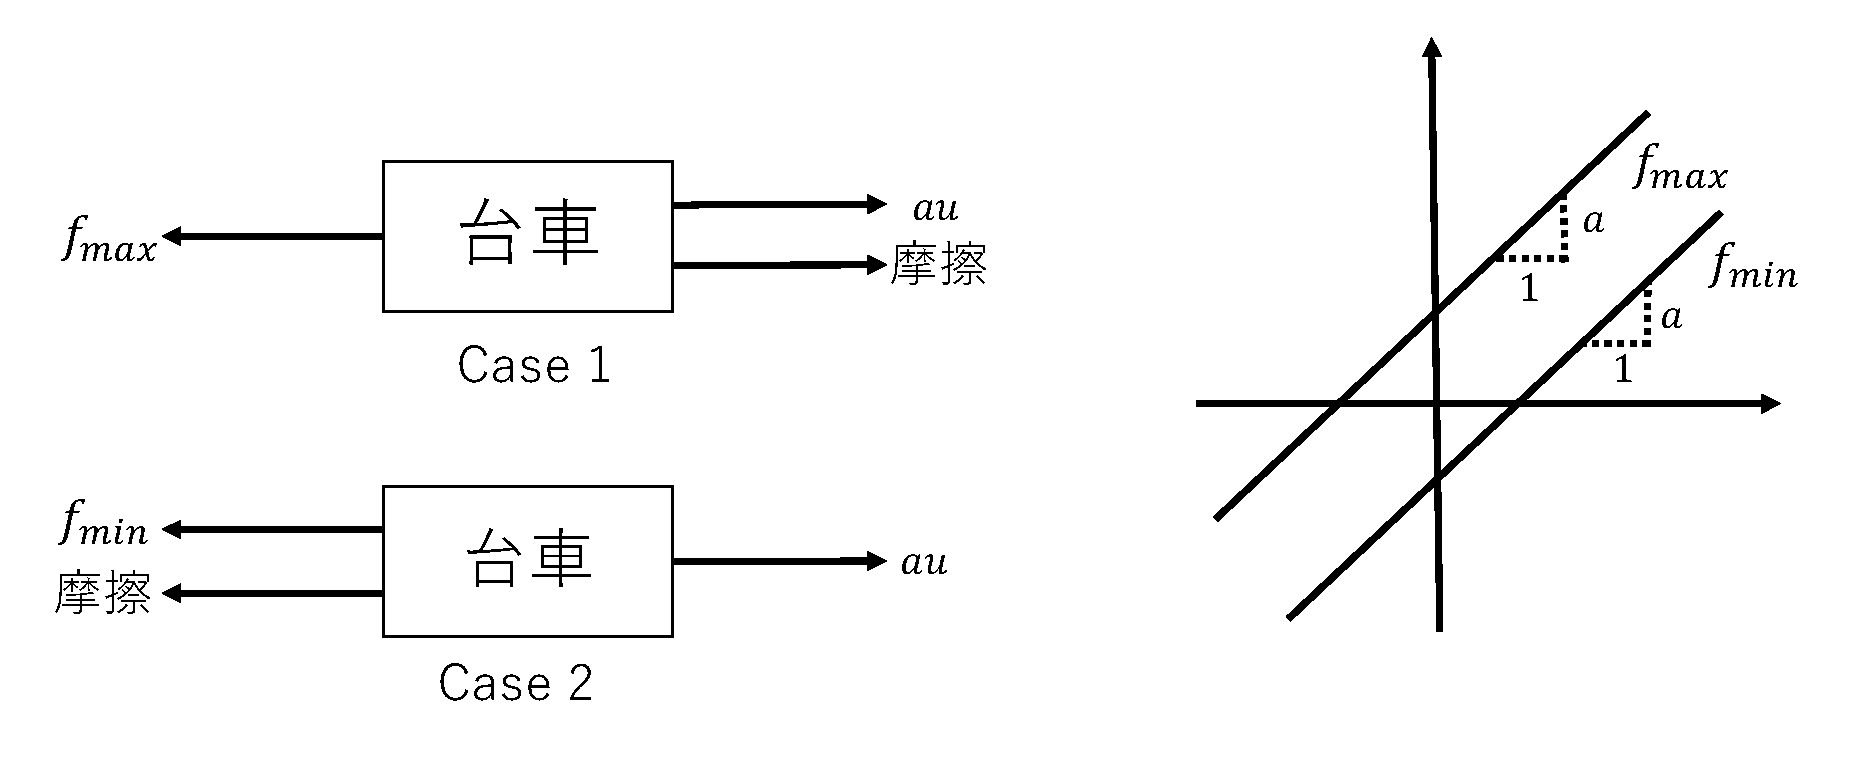
\includegraphics[width=1.0\linewidth]{gazo/ParameterA.eps}
		\caption{パラメータaの決定}
		\label{image:parameterA}
	\end{figure}
	以下に測定した結果を示す。
	\[
		a=0.062[\rm{Kg/V}] = 6.1E-1[\rm{N/V}
	]\]
\subsection{Mとfの測定}
	
\subsection{Jとcの測定}
	振子を自由振動させることにより、$J$と$c$を測定できる。その数式モデルは鉛直下向きを基準として
	\begin{equation}
		(J + ml^{2})\ddot{\theta} - mgl\sin{\theta} + c\dot{\theta} = 0
		\label{eq:Para1}
	\end{equation}
	\begin{equation}
		y_{2} = c_{2}\theta
	\label{eq:Para2}
	\end{equation}
	で与えられる。$\theta$を微小範囲で考えると、(\ref{eq:Para1}),(\ref{eq:Para2})式は
	\begin{equation}
		\ddot{y}_{2} + 2\zeta\omega_{n}\dot{y}_{2} + \omega_{n}^{2}y_{2} = 0
	\end{equation}
	ただし、
	\begin{equation}
		\zeta = \frac{c}{2\sqrt{mgl\left(J + ml^{2}\right)}} 
		,\ \  \omega_{n} = \sqrt{\frac{mgl}{J+ml^{2}}}
	\end{equation}
	のように書くことができる。この解は
	\[0<\zeta<1\]
	のとき、減衰振動となり
	\[
		y_{2}(t) = \frac{y_{2}(0)}{\sqrt{1-\zeta^{2}}}\exp{(-\omega_{n}\zeta t)}
	  	\sin{(\omega_{n}\sqrt{1-\zeta^{2}}t + \phi)}
	\]
	ただし
	\[
		\phi = \tan^{-1}{\frac{\sqrt{1-\zeta^2}}{\zeta}}
	\]
	で与えられる。
	\begin{figure}[H]
		\centering
		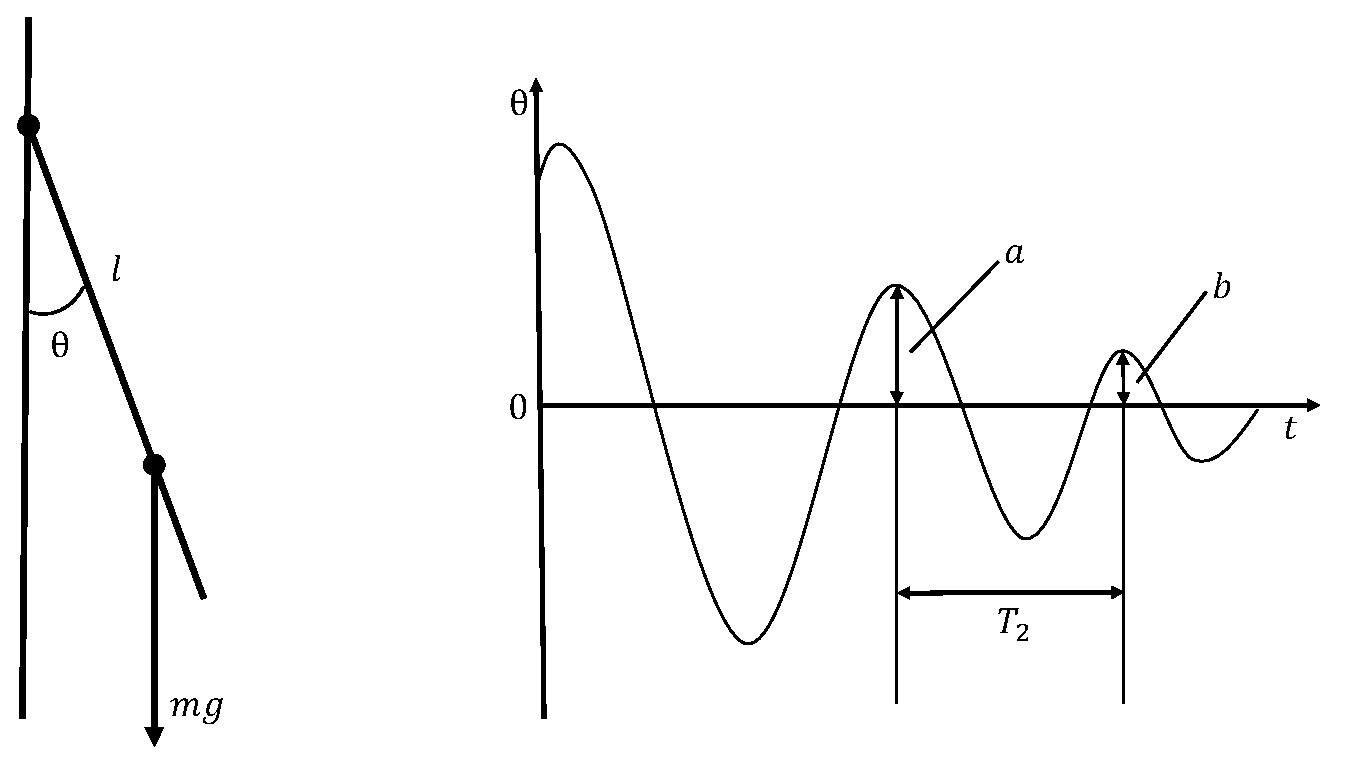
\includegraphics[width=1.0\linewidth]{gazo/ParameterJC.eps}
		\caption{$J$と$c$の測定}
		\label{image:parameterJC}
	\end{figure}
	\par
	いま、減衰振動の周期を$T_{2}$とし、時刻$t_{1}$と時刻$t_{2} = t_{1}+T_{2}$において波形
	$y_{2}(t)$の山が隣合うものとする。このときの振幅の減衰比は
	\[
		\frac{|y_{2}(t_{2})|}{|y_{2}(t_{1})|} = \exp{(-\lambda)}
	\]
	ただし
	\begin{equation}
		\lambda = \frac{2\pi\zeta}{\omega_{n}\sqrt{1-\zeta^2}}
	\end{equation}
	となる。この$\lambda$は対数減衰比と呼ばれる。また
	\[
		T_{2} = \frac{2\pi}{\omega_{n}\sqrt{1-\zeta^{2}}}
	\]
	が成り立つ。したがって、$J$と$c$は
	\begin{equation}
		J=\frac{mglT_{2}^{2}}{4\pi^{2}+\lambda^{2}}-ml^{2},\ \ 
		c=\frac{2\lambda(J+ml^{2})}{T_{2}}
	\end{equation}
	のように与えられる。\\
	以下に測定した結果を示す。
	\[
		J=2.5E-4[\rm{khm^{2}}]
	\]
	\[
		c=5.4E-5[\rm{kgm^{2}/s}]
	\]
	
\subsection{$c_1$と$c_2$の測定}
	$c_1$と$c_2$に関しては
	\[
		c_1 = 1.0 [\rm{V/m}]
	\]
	\[
		c_2 = 1.0[\rm{V/rad}]
	\]
	というようにソフトウェアに設定してあるものを使った。
\subsection{同定結果}
\section{パラメータの検証}
\section{設計(線形)モデルの決定}